\documentclass[12pt]{exam}
% \usepackage{pslatex}
\usepackage{graphicx}
\DeclareGraphicsExtensions{.jpg}
\usepackage{amsmath}
\usepackage{amsfonts}
\usepackage{enumerate}
\firstpageheader{}{}{}
\runningheader{\textbf{Math 251: Fall 2011}}
 {\ifcontinuation{\textbf{Problem continues}}{}}
 {\emph{Page \thepage~of \numpages}}
\runningheadrule
\runningfooter{}{\ifincomplete{continues on next page}{}}{}
\setlength{\parskip}{1.2ex}
\setlength{\parindent}{0pt}
\pagestyle{headandfoot}
\newcommand{\N}{\mathbf{N}}
\newcommand{\Z}{\mathbf{Z}}
\newcommand{\R}{\mathbf{R}}
\DeclareGraphicsExtensions{.pdf,.png,.jpg}
\begin{document}

% \printanswers
\addpoints

\noindent
\textbf{{\large Mathematics 251 \\ Exam 2}}
% \hfill Name: \underline{\hspace{0.5in}Answers\hspace{2in}}

\noindent
October 26, 2011  \hfill Name: \underline{\hspace{3in}}


\noindent
\textbf{Instructions}: This exam is closed book: you may refer to one $8.5 \times 11$ page of handwritten notes, but no electronic aids or
other printed references are permitted. \emph{Justification of all answers is required
for partial credit.} Unless
specifically directed, leave all answers in \textbf{exact form}, e.g.\
$\sqrt{3}$ instead of~1.732 and $\pi/2$ instead of~$1.57$.

Show all pertinent work. \emph{Correct answers without accompanying work will receive little or no credit.} Results from homework or from class can be cited freely. It is in your interest to display your solution in a
clear, readable fashion. Note that standards of justification are not as high as for homework.

If your work continues onto the back of another page, please indicate
this. Check and make sure you have all of the pages in the
exam; there should be \numpages, including this one. If you have a
question, please raise your hand.

Be sure to read all questions carefully and completely.

\vspace*{1.0in}

\begin{center}
\combinedgradetable[h]
\end{center}

\vspace*{0.5in}

\begin{center}
{\Large \emph{Good luck!}}
\end{center}

\newpage

\begin{questions}
\pointsinmargin

\question Evaluate the indicated partial derivatives of the functions below. Recall that~$f_x$ denotes~$\frac{\partial f}{\partial x}$. If you use the equality of mixed partials, indicate this with a note at the appropriate point in the calculation.
\[
    f(x,y) = \sin(x^2-xy+y^3), \quad g(x,y,z) = e^{1/z} (x^2 y + \tan(xy)), \quad h(x,t) = \frac{1}{\sqrt{t}} e^{-x^2/4t}
\]
\begin{parts}

\part[8] Find $f_x$ and $f_{xy}$.

\vspace*{2.5in}

\part[8] Find $g_x$ and $g_{xz}$.

\vspace*{2.5in}

\part[8] Find $h_x$ and $h_{xt}$.
\end{parts}
\newpage

\question[12] Consider the function $f \colon \R \to \R$ given by $f(x) = e^{x^2-x}$. What is the curvature of its graph at the point $(0,1)$?

\vspace*{\stretch{1}}

\question[12] Consider the parametric curve $\mathbf{r}(t) = \langle e^{-2t},2t^2,e^{2t} \rangle$. Find the unit tangent vector $\mathbf{T}(2)$ and the tangential component of acceleration $a_{\mathbf{T}}$ (that is, find $a_{\mathbf{T}}$ where $\mathbf{a}(2) = a_{\mathbf{T}} \mathbf{T}(2)$).

\vspace*{\stretch{1}}

\newpage

\question Furious at life's injustices, Dr.\ Rosoff hurls his empty coffee mug at an angle of $\pi/12$ (measured up from the ground). It lands 125 meters (measured horizontally) from him (what an arm!). It may help to recall that in this situation, the throwing angle $\theta$, initial speed $v_0$, and total distance $x$ are related by the equation $x = (v_0^2/g) \sin 2\theta$. \textbf{In this problem, use} $g~=~10$~m/s$^2$.

\begin{parts}

\part[4] With what initial speed was the fearsome projectile discharged?

\vspace*{\stretch{1}}

\part[12] Make an appropriate choice of coordinates and find a vector-valued function $\mathbf{r}(t)$ that describes the position of the mug, assuming the fateful launch occurs at $t = 0$.

\vspace*{\stretch{2}}

\part[4] What is the mug's maximum height above the fertile earth, who someday shall shelter us all in her boundless embrace?

\vspace{\stretch{1}}

\end{parts}

\newpage

\question Consider the function $f(x,t)$ defined on the half-infinite strip $\{ (x,t) \in \R^2 : -6 \leq x \leq 6,\; t > 0 \}$ by the formula
\[
f(x,t) = t^{-1/2}e^{-x^2/t}.
\]
\begin{parts}

\part[6] Which of the following is a contour plot for $f(x,t)$? No justification is necessary, just select the (unique) correct answer.

\vspace{2ex}

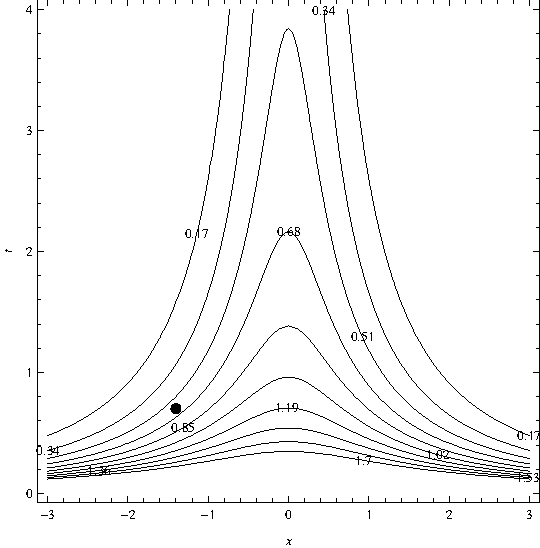
\includegraphics[scale=0.75]{F2011_exam_2_fig2} \hspace{1.6em}
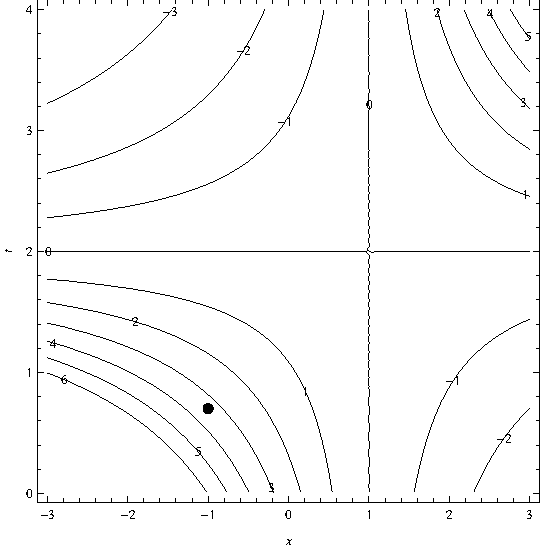
\includegraphics[scale=0.75]{F2011_exam_2_fig4} \\

\vspace{2ex}

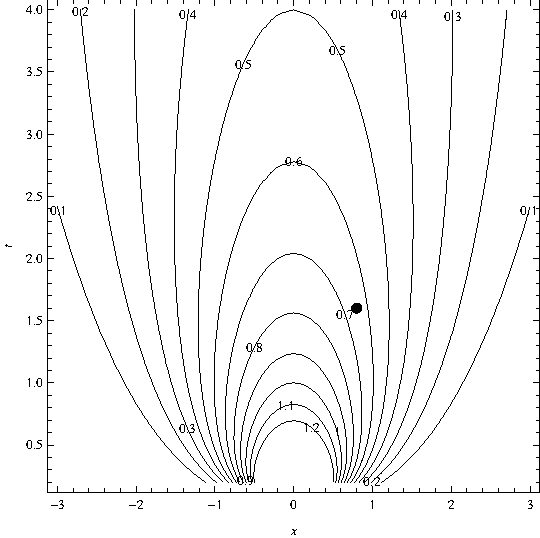
\includegraphics[scale=0.75]{F2011_exam_2_fig1} \hspace{1.6em}
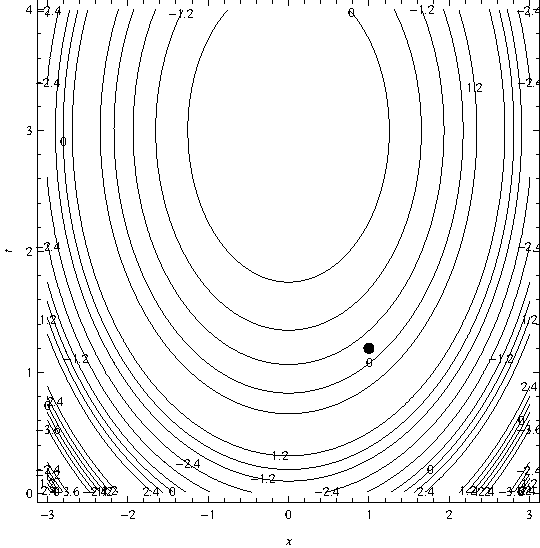
\includegraphics[scale=0.75]{F2011_exam_2_fig3}

\vspace{2ex}

\part[6] Consider the marked point in the figure you selected. Use the contours to sketch the path beginning at this point that moves ``uphill'' most steeply (it doesn't have to be a very long path: if it crosses two contours that is sufficient).

\end{parts}
\newpage

\question\label{prob:limit} Consider the function $f \colon \R^2 - \{ (0,0) \}$ defined by $f(x,y) = \dfrac{3x^2 y}{x^2+y^2}$. This problem investigates the behavior of this function near the origin.

\begin{parts}

\part[8] By substituting $mx$ for $y$ and taking an appropriate one-variable limit, show that $f(x,y)$ approaches $0$ along all (nonvertical) rays through the origin. (The limit is 0 along the vertical rays as well, but you do not need to show this.) What does this tell you about ${\displaystyle \lim_{(x,y) \to (0,0)} f(x,y)}$?

\vspace{\stretch{1}}

\part[4] Show that, if $y \ne 0$, $\dfrac{x^2}{x^2+y^2} \leq 1$. (This inequality is true generally and doesn't depend on any considerations about $f$.)

\vspace{\stretch{1}}

\newpage

\part[4] Use the previous part to show that $|f(x,y)| \leq 3 |y|$. \emph{Hint.} Start your calculation with $|f(x,y)|$ and use a combination of algebraic manipulations and references to the previous parts to build a chain of inequalities $|f(x,y)| \leq \cdots \leq 3|y|$.

\vspace{\stretch{2}}

\part[4]\label{part:squeeze} Use the previous part and the Squeeze Theorem\footnote{Recall the Squeeze Theorem: if $g_{\ell}$, $g$, $g_{r}$ are functions with $g_{\ell}(x,y) \leq g(x,y) \leq g_{r}(x,y)$ then all three functions have the same limit at $(a,b)$, provided the limits of $g_{\ell}$ and $g_{r}$ at $(a,b)$ exist and are equal.} to compute ${\displaystyle \lim_{(x,y) \to (0,0)} f(x,y)}$.

\vspace{\stretch{1}}

\bonuspart[4] Is $f$ continuous at $(0,0)$? Explain, referring to the definition of continuity as necessary.

\vspace{\stretch{1}}

\end{parts}

\newpage

\bonusquestion[8] Prove the limit result of part~\ref{part:squeeze} of problem~\ref{prob:limit} without using the Squeeze Theorem, directly from the $\varepsilon$-$\delta$ definition of limit.

\vspace{\stretch{3}}

\bonusquestion[3] Recall that the \emph{osculating circle} to a curve at a point $P$ is the unique circle tangent to the curve at $P$ of radius $1/\kappa(P)$. Also, the plane containing the osculating circle is called the \emph{osculating plane}. What does the word ``osculating'' mean in \emph{non-mathematical} contexts?

\vspace{\stretch{1}}

\end{questions}

\end{document} 